\documentclass{article}
\usepackage[utf8]{inputenc}
\usepackage{multirow}
\usepackage{multicol}
\usepackage{longtable}
\usepackage{graphicx}
\usepackage{color}

\title{Trabalho Final}
\author{Bruna Silva}
\date{28/02/2021}

\begin{document}
\maketitle

\section{\textcolor{blue}{Introdução}}
\noindent
\textcolor{red}{Lorem ipsum dolor sit amet, consectetur adipiscing elit. Suspendisse venenatis
semper rutrum. Ut viverra dignissim efficitur. Proin scelerisque congue dui
vitae vehicula. Duis aliquam eget eros nec luctus. Phasellus et nisi nec risus
molestie cursus eget eget ligula. Morbi eu efficitur metus. Vivamus nec tincidunt
ante, ac viverra ligula. Nunc eu nisl at ante molestie placerat ac non mauris.
Maecenas laoreet tristique sollicitudin. Nam imperdiet ligula ut finibus laoreet.
}

\textbf{Integer consequat felis eu nisi auctor laoreet. Curabitur metus
risus, ornare vitae urna vel, blandit mollis mauris. Aliquam justo
ipsum, tristique rhoncus lobortis in, pharetra at sapien. Nullam at
bibendum enim, porttitor vestibulum lacus. Donec id lacus nec ligula
rutrum convallis non non neque. Praesent venenatis nec nisi vitae
venenatis. Vivamus ut eros bibendum, fringilla massa eu, posuere
libero.}

\textit{Integer finibus metus eros, vitae interdum quam euismod et. Pellentesque
habitant morbi tristique senectus et netus et malesuada fames ac turpis egestas.
Praesent dictum nisl a arcu efficitur rutrum. Nunc condimentum lobortis enim
quis vehicula. Maecenas ornare, leo eu auctor feugiat, risus enim vestibulum
massa, non egestas arcu sapien in libero. Nulla facilisis enim eu tempor bibendum. Cras eget velit eu sapien maximus mollis. Donec dignissim odio orci, sit
amet luctus enim egestas vitae. Cras euismod cursus diam, ut commodo augue
fermentum a. Mauris consectetur purus augue, ut feugiat arcu rhoncus in. Sed
id massa at ante facilisis pellentesque. Morbi est nunc, finibus condimentum
faucibus sit amet, aliquam ac urna. Morbi vitae magna sed ex vulputate dapibus
in in enim. Maecenas nec hendrerit est. Integer hendrerit nisl orci, gravida sodales velit dapibus eu. Pellentesque id condimentum magna, ut porttitor lacus.
}

\subsection{Subseção}
Aenean lacus augue, tincidunt a tempus in, ultrices molestie mi. Quisque congue
fringilla magna vel lobortis. Suspendisse ut nisl mollis, congue libero eu, commodo mauris. In lacus tellus, fringilla eu neque in, pulvinar varius sem. Donec
vitae leo dignissim, lobortis leo sodales, blandit ipsum. Mauris imperdiet arcu
eget metus finibus fermentum eget a quam. Pellentesque felis est, vestibulum ut turpis nec, dignissim elementum nulla. Nullam vel sollicitudin augue. Aliquam
nec mauris lobortis, suscipit ipsum id, ultrices sapien. Phasellus dictum purus
in felis ultrices venenatis. Mauris dictum pretium tortor. Fusce augue metus,
dapibus at cursus ut, gravida in neque. Donec bibendum eros diam. Nunc
sapien neque, rhoncus sit amet accumsan id, volutpat congue nisi.

Suspendisse vestibulum ornare diam lobortis gravida. Donec ornare quis
tortor id posuere. Etiam feugiat sapien a risus finibus, nec sodales nunc rhoncus.
Mauris molestie commodo arcu, sit amet mollis erat porta quis. Quisque a est
ut eros sagittis maximus. Curabitur a facilisis sem. Aliquam feugiat odio sit
amet purus feugiat, vel egestas tortor rutrum.

\section{Figuras}
\begin{figure}[htpb]
    \centering
    \begin{tabular}{cccc}
        \multirow{2}{*}{\rotatebox[origin=c]{90}{\textbf{rota rota rota rota}}} & &\\
         &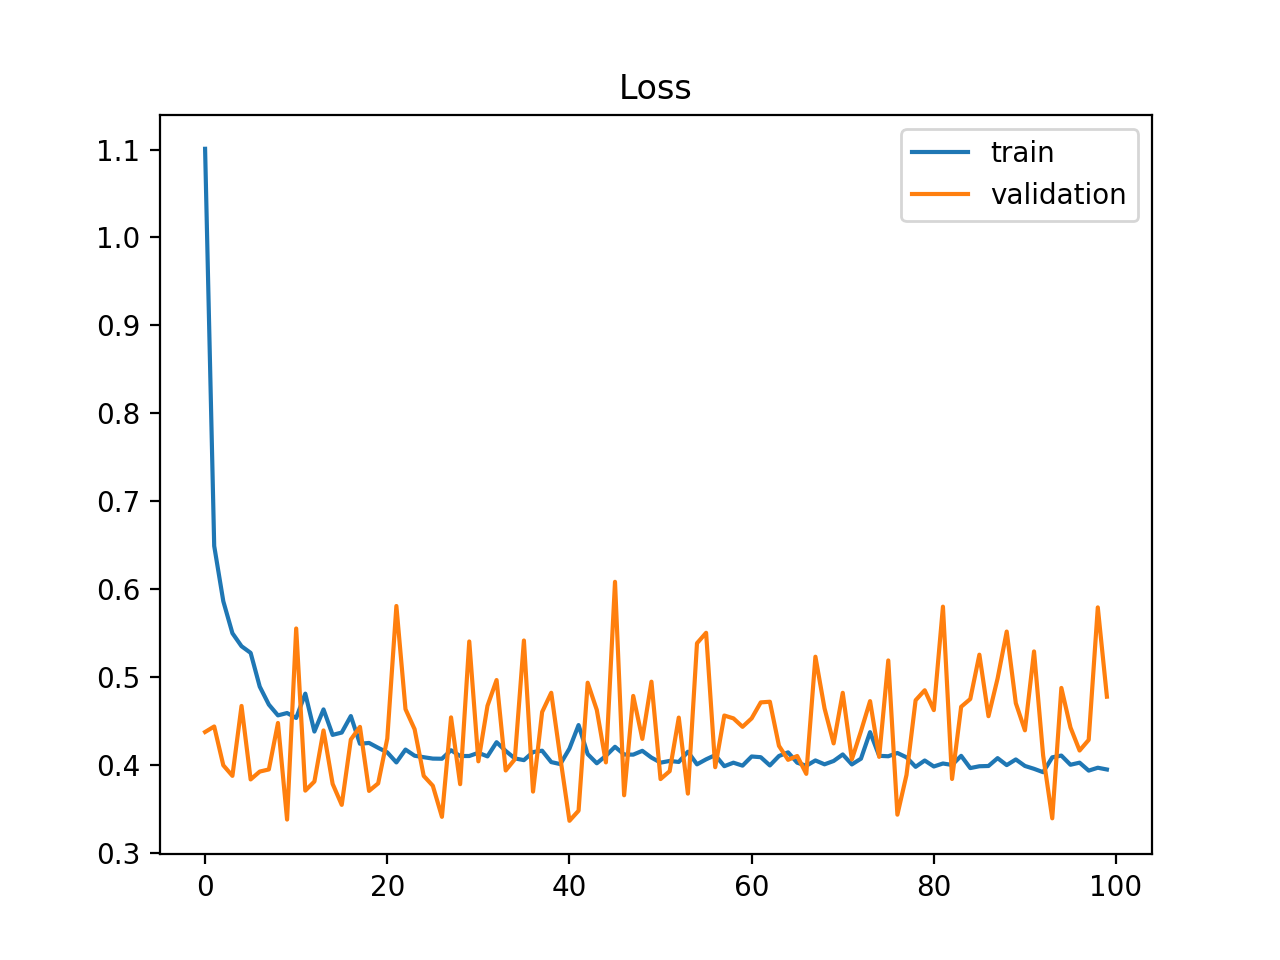
\includegraphics[scale=0.3]{imagens/imagem-1.png}& 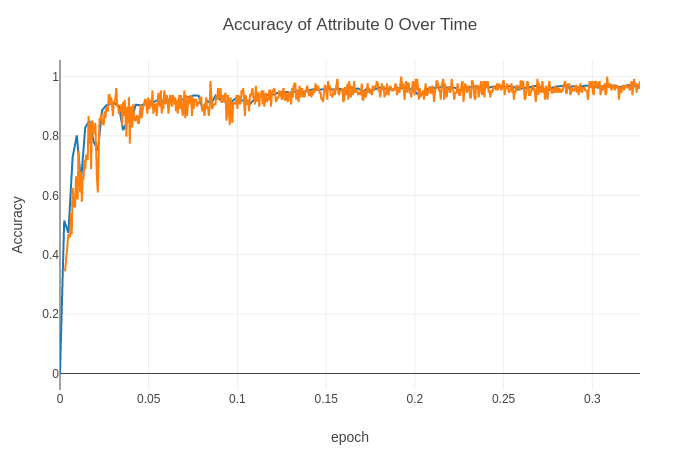
\includegraphics[scale=0.2]{imagens/image-2.png} \\ 
         &\textbf{(A)} & \textbf{(B)} 
    \end{tabular}
    \caption{Figuras lado a lado}
    \label{fig:my_label}
\end{figure}

\begin{figure}[htpb]
    \centering
    \begin{tabular}{cccc}
         
\includegraphics[scale=0.7]{imagens/phdcomics.png} \\
    \end{tabular}
    \caption{Figura 3}
    \label{fig:my_label}
\end{figure}

\section{Tabelas}
\begin{longtable}{p{6.5cm}p{3.5cm}p{0.3cm}p{0.5cm}}
     \caption{Tabela Gigante}
     \label{tab;gigante}\\
     
     \hline
     \multicolumn{1}{c}{\textbf{Dados 1}} &
     \multicolumn{1}{c}{\textbf{Dados 2}} &
     \multicolumn{1}{c}{\textbf{Dados 3}} &
     \multicolumn{1}{c}{\textbf{Dados 4}} \\
     \hline
     \endfirsthead
     
     \hline \multicolumn{4}{r}{{Continua na próxima página}} \\
     \hline
     \hline
          \endfoot
          
      \multicolumn{4}{c}{{\bfseries \tablename\ \thetable{} -- comtinuação da página anterior}} \\
      \hline
      \multicolumn{1}{c}{\textbf{Referencia}}&\multicolumn{1}{c}{\textbf{Editora}}&\multicolumn{1}{c}{\textbf{h5}}&\multicolumn{1}{c}{\textbf{SJR}}\\
      \hline
      \endhead
      
      \hline \hline
      \endlastfoot
      
          \citet{Lorem}                 & Ipsum                  & dolor & sit \\
            \citet{Lorem}                 & Ipsum                  & dolor & sit \\
            \citet{Lorem}                 & Ipsum                  & dolor & sit \\
            \citet{Lorem}                 & Ipsum                  & dolor & sit \\
            \citet{Lorem}                 & Ipsum                  & dolor & sit \\
            \citet{Lorem}                 & Ipsum                  & dolor & sit \\
            \citet{Lorem}                 & Ipsum                  & dolor & sit \\
            \citet{Lorem}                 & Ipsum                  & dolor & sit \\
            \citet{Lorem}                 & Ipsum                  & dolor & sit \\
            \citet{Lorem}                 & Ipsum                  & dolor & sit \\
            \citet{Lorem}                 & Ipsum                  & dolor & sit \\
            \citet{Lorem}                 & Ipsum                  & dolor & sit \\
            \citet{Lorem}                 & Ipsum                  & dolor & sit \\
            \citet{Lorem}                 & Ipsum                  & dolor & sit \\  \citet{Lorem}                 & Ipsum                  & dolor & sit \\
            \citet{Lorem}                 & Ipsum                  & dolor & sit \\
            \citet{Lorem}                 & Ipsum                  & dolor & sit \\
            \citet{Lorem}                 & Ipsum                  & dolor & sit \\
            \citet{Lorem}                 & Ipsum                  & dolor & sit \\
            \citet{Lorem}                 & Ipsum                  & dolor & sit \\
            \citet{Lorem}                 & Ipsum                  & dolor & sit \\
            \citet{Lorem}                 & Ipsum                  & dolor & sit \\
            \citet{Lorem}                 & Ipsum                  & dolor & sit \\
            \citet{Lorem}                 & Ipsum                  & dolor & sit \\
            \citet{Lorem}                 & Ipsum                  & dolor & sit \\
            \citet{Lorem}                 & Ipsum                  & dolor & sit \\
            \citet{Lorem}                 & Ipsum                  & dolor & sit \\
            \citet{Lorem}                 & Ipsum                  & dolor & sit \\
            \citet{Lorem}                 & Ipsum                  & dolor & sit \\
            \citet{Lorem}                 & Ipsum                  & dolor & sit \\
            \citet{Lorem}                 & Ipsum                  & dolor & sit \\
            \citet{Lorem}                 & Ipsum                  & dolor & sit \\
            \citet{Lorem}                 & Ipsum                  & dolor & sit \\
            \citet{Lorem}                 & Ipsum                  & dolor & sit \\
            \citet{Lorem}                 & Ipsum                  & dolor & sit \\
            \citet{Lorem}                 & Ipsum                  & dolor & sit \\
            \citet{Lorem}                 & Ipsum                  & dolor & sit \\
            \citet{Lorem}                 & Ipsum                  & dolor & sit \\
            \citet{Lorem}                 & Ipsum                  & dolor & sit \\
            \citet{Lorem}                 & Ipsum                  & dolor & sit \\
            \citet{Lorem}                 & Ipsum                  & dolor & sit \\
            \citet{Lorem}                 & Ipsum                  & dolor & sit \\
            \citet{Lorem}                 & Ipsum                  & dolor & sit \\
            \citet{Lorem}                 & Ipsum                  & dolor & sit \\
            \citet{Lorem}                 & Ipsum                  & dolor & sit \\
            \citet{Lorem}                 & Ipsum                  & dolor & sit \\
            \citet{Lorem}                 & Ipsum                  & dolor & sit \\
            \citet{Lorem}                 & Ipsum                  & dolor & sit \\
            \citet{Lorem}                 & Ipsum                  & dolor & sit \\
            \citet{Lorem}                 & Ipsum                  & dolor & sit \\
            \citet{Lorem}                 & Ipsum                  & dolor & sit \\
            \citet{Lorem}                 & Ipsum                  & dolor & sit \\
            \citet{Lorem}                 & Ipsum                  & dolor & sit \\
            \citet{Lorem}                 & Ipsum                  & dolor & sit \\
            \citet{Lorem}                 & Ipsum                  & dolor & sit \\
            \citet{Lorem}                 & Ipsum                  & dolor & sit \\
            \citet{Lorem}                 & Ipsum                  & dolor & sit \\
            \citet{Lorem}                 & Ipsum                  & dolor & sit \\
            \citet{Lorem}                 & Ipsum                  & dolor & sit 
\end{longtable}

\begin{table}[!htpb]
    \centering
    \begin{tabular}{|c|c|c|c|}
         \hline
         \textbf{Dado 1} & \textbf{Dado 2} & \textbf{Dado 3} & \textbf{Dado 4} \\
         \hline
         
         \multicolumn{2}{|c|}{Gastos} & teste & teste\\
         \hline
         
         Dado Inicial & \multicolumn{3}{|c|}{Gastos} \\
         \hline
         
         \multicolumn{4}{|c|}{Gastos} \\
         \hline
    \end{tabular}
    \caption{Minha legenda para uma tabela com colunas e linhas 'mescladas'.}
    \label{tab:my_label}
\end{table}

\begin{table}[htb]
    \centering
    \begin{tabular}{c|c}
         \textbf{Unidade} & \textbf{Comprimento} \\
         \hline \\
         
         mm & valor normal em milímetros \\
         cm & valor normal em centímetros \\
         in & valor em polegadas \\
         pt & 1/3 de um milímetro \\
         em & largura e altura "M" \\
         ex & largura e altura "x"
    \end{tabular}
    \caption{Unidades de Medida padrões do \LaTeX}
    \label{tab:my_label}
\end{table}

\section{Equações}
\begin{equation}
    x = \sum{3+4}
\end{equation} \\

\begin{equation}
    x = \frac{-b \pm \sqrt{b^2 - 4ac}}{2a}
\end{equation}

\section{Citações}
\textbf{Título do Artigo:} Machine learning for COVID-19—asking the right questions \cite{ZHANG2016}. \\

\textbf{Título do Artigo:} New machine learning method for image-based diagnosis of COVID-19 \cite{YASSIN2018}

\bibliographystyle{unsrt}
\bibliography{references}


\end{document}
